\chapter{実験}

\section{実験の設定}
\subsection{提案手法の概要}
提案手法のモデルについて述べる。実装はPythonを使用言語とし、PyTorchをフレームワークとして用いた。提案手法には2層のグラフ畳み込みネットワークを用いた。畳み込み層では過学習を防ぐためのdropoutを用い、活性化関数として、隠れ層ではReLU関数、出力層としてSoftmax関数を用いた。また最適化にはAdam\cite{KingmaB14Adam}を用いた。
また提案手法や比較手法で用いるGCNのハイパーパラメータは表\ref{tab:gcn_hyperparams}に示した通り、ノード分類とリンク予測では異なる値を用いた。

\subsection{データセット}
実験には引用ネットワーク(Cora,Citeseer)\cite{sen2008col}と共購買ネットワーク(Amaphoto,Amacomp)\cite{amazondata2015}の計4種類のデータセットを用いた。
\begin{itemize}
\item 引用ネットワーク(Cora, Citeseer):\\
論文をノード、引用をエッジとしたネットワークである。論文をbag-of-words表現で表し、その単語が含まれる場合を1、それ以外を0としてベクトル表現で表したものを特徴量としている。論文の種類をラベルとして各ノードに割り当てている。
\item 共購買ネットワーク(Amaphoto, Amacomp):\\
商品をノード、利用者が同時に購入しやすい商品をエッジで表したネットワークである。その商品に対するユーザーのレビューをbag-of-words表現で表したものを特徴量としている。商品の種類をラベルとして各ノードに割り当てている。
\end{itemize}

4種類のデータセットの詳細は以下の表\ref{tab:statdata}で示した。データセットは比較手法の条件と同様になるように、有向エッジを全て無向エッジに変換して実験を行った。また実験を行うためにデータセットに人工的に欠損値を含むような実装をした。人工的な欠損値として以下の3種類の欠損パターンを用いた。

\begin{itemize}
\item Unirom randomly missing:\\
全ての特徴量を等しい確率で欠損させたケースである。
\item Biased randomly missing:\\
特徴量の種類ごとにランダムに特徴量を選択し、選択された特徴量の欠損率を90\%に、選択されなかった特徴量の欠損率を10\%にしたケースである。
\item Structurally missing:\\
ノード全体の集合から一様ランダムにノードを選択し、選択されたノードの特徴量を全て欠損させるケースである。
\end{itemize}

図\ref{fig:ex_missing_graph}は特徴量にそれぞれの欠損パターンを適用させた例を示している。この例は欠損率を50\%にした例である。またグラフにおいては縦軸をノード番号、横軸を特徴量番号として考えることができる。(a)のUniform randomly missingは全ての特徴量の中からランダムで50\%の特徴量が欠損している。(b)のBiased randomly missingでは特徴量a,b,cでは90\%のノードを欠損値としており、d,e,fでは10\%のノードを欠損値としている。(c)のStructurally missingではノード1,4,5,7の全ての特徴量を欠損値であり、それ以外の全ての特徴量を観測値となっている。

\begin{table}[!b]
    \centering
    \caption{GCNのハイパーパラメータ設定}
    \scalebox{.97}{
    \begin{tabular}{c|ccccc} \toprule
         & 学習率 & L2正則化項 & ドロップアウト率 & エポック数 & patience \\ \midrule
        \begin{tabular}{c}
            ノード分類\\(Cora、Citeseer)
        \end{tabular}& 0.01 & $5\cdot10^{-4}$ & 0.5 & 200 & 10 \\
        \begin{tabular}{c}
            ノード分類\\(AmaPhoto、AmaComp)
        \end{tabular} & 0.005 & $5\cdot10^{-5}$ & 0.5 & 10000 & 100 \\
        リンク予測 & 0.01 & 0 & 0 & 200 & - \\
        \bottomrule
    \end{tabular}
    }
    \label{tab:gcn_hyperparams}
\end{table}


\begin{figure}
	\subfigure[Uniform randomly missing]{%
		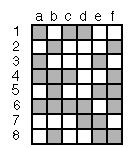
\includegraphics[clip, width=0.33\columnwidth]{figures/random_uniform.pdf}}%
	\subfigure[Biased randomly missing]{%
		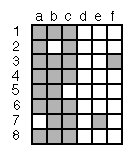
\includegraphics[clip, width=0.33\columnwidth]{figures/random_bias.pdf}}%
    \subfigure[Structurally missing]{%
		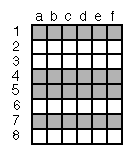
\includegraphics[clip, width=0.33\columnwidth]{figures/random_struct.pdf}}%
	\caption{欠損率50\%のときの欠損パターン例。8ノード(ノード番号1 -- 8)、6次元(a -- f)。白いセルは観測されている要素を、黒いセルは欠損している要素を表す。\cite{taguchi2021graph}より引用。}
	\label{fig:ex_missing_graph}
\end{figure}




\begin{table}[!t]
    \centering
    \caption{データセットの詳細情報。ただし、訓練ラベル数、検証ラベル数、テストラベル数はそれぞれ半教師ありノード分類で用いるラベルの数に対応する。\cite{taguchi2021graph}より引用}
    \label{tab:statdata}
    \begin{tabular}{l|cccc} \toprule
        データセット & Cora & Citeseer & AmaPhoto & AmaComp\\ \midrule
        ノード数 & 2,708 & 3,327 & 7,650 & 13,752\\
        エッジ数 & 5,429 & 4,732 & 143,663 & 287,209\\
        特徴量の次元 & 1,433 & 3,703 & 745 & 767\\
        クラス数 & 7 & 6 & 8 & 10\\
        訓練ラベル数 & 140 & 120 & 320 & 400\\
        検証ラベル数 & 500 & 500 & 500 & 500\\
        テストラベル数 & 1,000 & 1,000 & 6,830 & 12,852\\
        \bottomrule
    \end{tabular}
\end{table}

\subsection{比較手法}
比較手法では代入法を用いた9つの手法と欠損データを直接学習する1つの手法を用いる。
\begin{itemize}
    \item \textsc{MEAN} \cite{GarciaLaencina2010}: 
        特徴量の種類ごとに観測値のみで平均値を調べ、特徴量の種類ごとの欠損値にその値を代入する。
    \item \textsc{K-NN} \cite{batista2002study}:
        K近傍法を用いて、それぞれのノードごとの特徴量ベクトルに類似した特徴量ベクトルK個の平均により欠損値を代入法により補完する。
    \item \textsc{MFT} \cite{koren2009mf}:
       Matrix Factorizationを用いて全体の特徴量行列を2つの低ランク行列に分解し、再構成した値により欠損値を補完する。
    \item \textsc{SoftImp} \cite{mazumder2010soft}:
        特徴量行列を特異値分解することで低ランクの近似を行い行列補完する。
    \item \textsc{MICE} \cite{buuren2010mice}:
        多重代入法\cite{rubin2004multiple}の1つである。連鎖方程式に基づいて得られた複数のデータを用いて欠損値を補完する。
    \item \textsc{MissForest} \cite{Stekhoven2011missforest}:
        ランダムフォレストを用いて欠損値を補完する。
    \item \textsc{VAE} \cite{kingma2013auto}:
        変分オートエンコーダを用いる手法である。欠損値を潜在変数を用いて補完する。
    \item \textsc{GAIN} \cite{yoon2018gain}:
        敵対的生成ネットワークを用いて欠損値補完する。
    \item \textsc{GINN} \cite{spinelli2019ginn}:
        Graph Denoising AutoEncodeを用いて欠損値補完する。
    \item \textsc{GCNmf} \cite{taguchi2021graph}:
        混合ガウスモデル(GMM)を用いて欠損値を確率分布で表現し、欠損値を含む特徴量を用いて直接学習する。
\end{itemize}

\section{ノード分類}
提案手法の評価を行うために半教師ありノード分類の精度を調べた。実験はUniform randomly missing, Biased randomly missing, Structurally missingの3種類の欠損パターンを用いた。また、欠損率は10\%から90\%までを10\%づつ変化させた9種類の欠損率を用いた。ラベルの訓練/検証/テストの割合はCora,Citeseerではクラスごとに20ノードを訓練データとして選択し、検証ラベル数は500,テストラベル数は1000で実験を行った。またAmaphoto,Amacompではクラスごとに40ノードを訓練データとして選択し、検証ラベル数は500,残りの全てのノードをテストラベルとしてで実験を行った。また実験は1つの欠損パターンで20回の実験を行い、それを5つの欠損パターンで行い平均することで精度を調べた。つまり合計で100回実験の平均を分類精度とした。

分類精度の指標はそのノードのラベルの正解率をAccuracyとして求めた。Accuracyは0から100までの値をとり、値が大きいほど精度が良いことを示す。実験のエポック数を100,000とし、その中でEarly Stoppingのpatienceを100とすることで学習を打ち切りにすることで過学習を防いだ。またGCNを用いる手法において隱れ層の次元数はCora,Citeseerで16、Amaphoto,Amacompで64に統一した。提案手法の1つであるGCN\_recursiveモデルの再帰回数は32回として実験を行った。

表\ref{table_cora}から表\ref{table_amacomp}はノード分類の精度を示している。欠損パターンと欠損値率毎のそれぞれの結果で最も良い精度を示している値を太字として示している。比較手法の中で、MICEのCora,Citeseerの結果と、MissForestのCiteseer,AmaCompは実験が24時間以内に正常終了しないため、値を空欄で示している。

また表の最下層の列で完全データの特徴量を用いて実験を行った場合のGCNの精度と、完全データの特徴量を用いる代わりに、隣接行列を単位行列として実験を行った場合のGCNの精度をGCN $(\mathbf{X} = \mathbf{I}_N)$として提示している。

表\ref{table_cora}から表\ref{table_amacomp}の結果から以下のような考察をすることができる。まずはデータセットごとの結果を考える。データセットCoraにおいては3つの欠損パターンにおいてほとんどの欠損率で提案手法のGCN\_recursiveモデルの精度が比較手法を上回っていることがわかる。データセットCiteseer,Amaphoto,Amacompにおいては、3つの欠損パターンにおいてほとんどの欠損率において提案手法であるGCN\_recursiveモデルと比較手法の1つであるGCN\_mfモデルが高い精度を示している。

実験の多くの欠損パターン/欠損率で提案手法が比較手法よりも高い精度を示した要因を考察する。代入法を用いた比較手法は欠損値補完にグラフ構造を用いていない。また欠損値を含む特徴量から直接学習を行う手法であるGCN\_mfモデルはGMMでの特徴量表現においてノード間の関係を考慮していない。一方、本研究の2つの提案手法はグラフ構造を用いて欠損値補完を行っている。そのため、GCNがノードの特徴量を近隣ノードの特徴量を用いて学習するようなグラフを用いるモデルであることを考慮すると、提案手法は比較手法に比べてよりGCNに適した欠損値補完をしていると考えられる。

またCoraデータセットで特に提案手法が高い精度を示している要因を考察する。CoraデータセットはAmaphotoやAmacompと比べて疎なグラフであり、特徴量の種類もCiteseerに比べると少なくなっている。そのため、特徴量1つ1つの情報が他のデータセットに比べると重要であると考えられる。そのためグラフ構造を用いてGCNに適した欠損値補完をすることが、他のデータセットと比べてより効果を発揮していると考えられる。

次に欠損率が高い場合の提案手法と比較手法の精度を比較し考察する。欠損率が90\%の場合の実験結果から考える。全てのデータセット、全ての欠損パターンにおいて、欠損率が90\%の場合は提案手法が比較手法よりも高い精度を示している。特にデータセットCoraのStructurally missingのケースにおいては提案手法は比較手法から33.38\%も改善している。この要因は、観測値が少ないケースでは観測値1つ1つの情報が重要であるため、観測値を用いて欠損値をGCNに適した方法で補完している提案手法の精度が高くなったと考えられる。

また図\ref{fig:rec_cora}から\ref{fig:rec_amacomp}までは提案手法であるGCN\_recursiveモデルの再帰回数によるノード分類の精度の変化を調べている。この図ではそれぞれCora,Citeseer,Amaphoto,Amacompの4種類データセットでUniform randomly missing, Biased randomly missing,Structually Missingの3種類の欠損パターンにおける欠損値が0.2,0.5,0.8での精度について示している。

全体的なグラフから、欠損率が0.2や0.5などあまり大きくない場合は再帰回数によって分類精度がほとんど変化しないことが分かる。この要因としては欠損率が少ない場合は観測値が多いために再帰回数が少なくても欠損値補完のためのアルゴリズムが収束するからであると考えられる。

一方、欠損率が0.8と大きい場合はデータセットCoraやCiteseerにおいては再帰回数が16以下などの少ない場合は再帰回数が32以上の場合に比べて精度が下がっている傾向があることが確認できた。データセットAmaphotoや Amacompにおいては欠損率が0.8の場合でも再帰回数による精度の変化はほとんど見られなかった。この要因としてはデータセットCoraやCiteseerに比べ、AmaphotoやAmacompは密なグラフであるため、ノードの平均次数が大きく欠損率が高い場合でも少ない再帰回数で特徴量が収束するからであると考えられる。

\begin{table}[!pt]
    \centering
    \caption{Coraデータセットにおけるノード分類の精度}
    \label{table_cora}
    \scalebox{.84}{
    \begin{tabular}{c|c|ccccccccc} \toprule
欠損パターン &  欠損率 & 10\% & 20\% & 30\% & 40\% & 50\% & 60\% & 70\% & 80\% & 90\%\\ \midrule
\multirow{13}{*}{\shortstack{Uniform\\Randomly\\Missing}} & \textsc{MEAN} & {80.96} & 80.41 & 79.48 & 78.51 & 77.17 & 73.66 & 56.24 & 20.49 & 13.22\\
& \textsc{K-NN} & 80.45 & 80.10 & 78.86 & 77.26 & 75.34 & 71.55 & 66.44 & 40.99 & 15.11\\
& \textsc{MFT} & 80.70 & 80.03 & 78.97 & 78.12 & 76.43 & 71.33 & 45.82 & 27.22 & 23.98\\
& \textsc{SoftImp} & 80.74 & 80.32 & 79.63 & 78.68 & {77.32} & {74.26} & {70.36} & {64.93} & 41.20\\
& \textsc{MICE} & -- & -- & -- & -- & -- & -- & -- & -- & --\\
& \textsc{MissForest} & 80.68 & 80.43 & {79.74} & {79.27} & 76.12 & 73.70 & 68.31 & 60.92 & 45.89\\
& \textsc{VAE} & 80.91 & {80.47} & 79.18 & 78.38 & 76.84 & 72.41 & 50.79 & 18.12 & 13.27\\
& \textsc{GAIN} & 80.43 & 79.72 & 78.35 & 77.01 & 75.31 & 72.50 & 70.34 & 64.85 & {58.87}\\
& \textsc{GINN} & 80.77 & 80.01 & 78.77 & 76.67 & 74.44 & 70.58 & 58.60 & 18.04 & 13.19\\
& \textsc{GCNmf} & 81.70 & \textbf{81.66} & 80.41 & 79.52 & 77.91 & 76.67 & 74.38 & 70.57 & 63.49\\
& \textsc{GCN\_neighbor} & 81.14 & 80.89 & 80.27 & 78.90 & 78.42 & 77.15 & 75.75 & 73.57 & 69.11 \\
& \textsc{GCN\_recursive} & \bf{82.04} & 81.64 & \bf{80.74} & \bf{79.87} & \bf{79.40} & \bf{78.86} & \bf{78.03} & \bf{76.86} & \bf{76.35} \\
\midrule
\multirow{13}{*}{\shortstack{Biased\\Randomly\\Missing}} & \textsc{Mean} & {81.22} & {80.37} & {78.95} & 77.46 & 75.94 & 72.44 & 53.14 & 20.39 & 13.40\\
& \textsc{K-NN} & 80.75 & 79.94 & 78.33 & 77.17 & 75.62 & 72.66 & 67.05 & 54.71 & 15.13\\
& \textsc{MFT} & 80.75 & 75.01 & 56.28 & 55.76 & 43.81 & 29.31 & 25.88 & 21.79 & 21.07\\
& \textsc{SoftImp} & 81.04 & 80.30 & 78.80 & {78.50} & {75.99} & 73.65 & 61.37 & 60.06 & 46.38\\
& \textsc{MICE} & -- & -- & -- & -- & -- & -- & -- & -- & --\\
& \textsc{MissForest} & 80.90 & 80.10 & 78.79 & 77.54 & 74.66 & 71.04 & 65.28 & 56.65 & 44.30\\
& \textsc{VAE} & 80.92 & 80.33 & 78.86 & 77.25 & 75.74 & 69.29 & 53.53 & 18.11 & 13.27\\
& \textsc{GAIN} & 80.68 & 79.62 & 78.54 & 77.41 & 75.84 & {73.82} & {69.18} & {63.99} & {59.41}\\
& \textsc{GINN} & 80.86 & 80.10 & 78.45 & 76.80 & 74.60 & 72.08 & 65.72 & 50.08 & 13.22\\
& \textsc{GCNmf} & \textbf{82.29} & \textbf{81.09} & 80.00 & 79.23 & 77.33 & 76.19 & 72.57 & 68.19 & 65.73\\ 
&\textsc{GCN\_neighbor}  & 81.51 & 80.23 & 78.29 & 78.54 & 76.09 & 74.68 & 74.54 & 72.49 & 70.21 \\ 
&\textsc{GCN\_recursive}  & 81.31 & 80.58 & \textbf{80.57} & \textbf{80.11} & \textbf{79.89} & \textbf{79.53} & \textbf{78.18} & \textbf{77.14} & \textbf{76.30} \\ 
\midrule
\multirow{13}{*}{\shortstack{Structurally\\Missing}} & \textsc{MEAN} & {80.92} & {80.40} & {79.05} & {77.73} & {75.22} & 70.18 & 56.30 & 25.56 & 13.86\\
& \textsc{K-NN} & 80.76 & 80.26 & 78.63 & 77.51 & 74.51 & {70.86} & {63.29} & 37.97 & 13.95\\
& \textsc{MFT} & 80.91 & 80.34 & 78.93 & 77.48 & 74.47 & 69.13 & 52.65 & 29.96 & 17.05\\
& \textsc{SoftImp} & 79.71 & 69.47 & 69.31 & 52.53 & 44.71 & 40.07 & 36.68 & 28.51 & {27.90}\\
& \textsc{MICE} & {80.92} & {80.40} & {79.05} & 77.72 & {75.22} & 70.18 & 56.30 & 25.56 & 13.86\\
& \textsc{MissForest} & 80.48 & 79.88 & 78.54 & 76.93 & 73.88 & 68.13 & 54.29 & 30.82 & 14.05\\
& \textsc{VAE} & 80.63 & 79.98 & 78.57 & 77.42 & 74.69 & 69.95 & 60.71 & 36.59 & 17.27\\
& \textsc{GAIN} & 80.53 & 79.78 & 78.36 & 77.09 & 74.25 & 69.90 & 61.33 & {41.09} & 18.43\\
& \textsc{GINN} & 80.85 & 80.27 & 78.88 & 77.35 & 74.76 & 70.58 & 59.45 & 29.15 & 13.92\\
& \textsc{GCNmf} & 81.65 & 80.77 & 80.67 & 79.24 & 77.43 & 75.97 & 72.69 & 68.00 & 55.64\\ 
& \textsc{GCN\_neighbor} & 81.77 & 81.10 & 79.82 & 79.63 & 78.47 & 76.17 & 74.49 & 71.06 & 62.36 \\ 
&  \textsc{GCN\_recursive} & \bf{81.97} & \bf{81.37} & \bf{80.68} & \bf{80.08} & \bf{78.73} & \bf{78.13} & \bf{78.23} & \bf{76.28} & \bf{74.21} \\ 
\midrule
\multicolumn{2}{c|}{GCN}& \multicolumn{9}{c}{81.49}\\ 
\multicolumn{2}{c|}{GCN $(\mathbf{X} = \mathbf{I}_N)$}& \multicolumn{9}{c}{63.22}\\
\bottomrule
    \end{tabular}
}
\end{table}


\begin{table}[!pt]
    \centering
    \caption{Citeseerデータセットにおけるノード分類の精度}
    \label{table_citeseer}
    \scalebox{.84}{
    \begin{tabular}{c|c|ccccccccc} \toprule
欠損パターン &  欠損率 & 10\% & 20\% & 30\% & 40\% & 50\% & 60\% & 70\% & 80\% & 90\%\\ \midrule
\multirow{13}{*}{\shortstack{Uniform\\Randomly\\Missing}} & \textsc{MEAN} & 69.88 & 69.62 & 68.97 & 65.12 & 54.62 & 37.39 & 18.29 & 12.28 & 11.88\\
& \textsc{K-NN} & 69.84 & 69.38 & 68.69 & 67.18 & 62.64 & 54.75 & 32.20 & 14.84 & 12.73\\
& \textsc{MFT} & 69.70 & 69.51 & 68.74 & 65.31 & 60.56 & 41.53 & 34.10 & 17.26 & 19.29\\
& \textsc{SoftImp} & 69.63 & 69.34 & {69.23} & {68.47} & {66.35} & \textbf{65.53} & 60.86 & {52.23} & 31.08\\
& \textsc{MICE} & -- & -- & -- & -- & -- & -- & -- & -- & --\\
& \textsc{MissForest} & -- & -- & -- & -- & -- & -- & -- & -- & --\\
& \textsc{VAE} & 69.80 & 69.39 & 68.54 & 64.13 & 50.91 & 29.62 & 18.45 & 12.49 & 11.00\\
& \textsc{GAIN} & 69.64 & 68.88 & 67.56 & 65.97 & 63.86 & 60.74 & 55.77 & 52.05 & {42.73}\\
& \textsc{GINN} & {70.07} & {69.79} & 68.87 & 68.14 & 63.21 & 43.61 & 20.74 & 13.26 & 11.31\\
& \textsc{GCNmf} & \textbf{70.93} & \textbf{70.82} & \textbf{69.84} & \textbf{68.83} & \textbf{67.03} & {64.78} & {60.70} & 55.38 & 47.78\\ 
&\textsc{GCN\_neighbor} & 68.37 & 67.11 & 66.48 & 65.37 & 63.43 & 61.27 & 59.50 & 56.18 & 51.50 \\
& \textsc{GCN\_recursive} & 69.34 & 68.82 & 68.25 & 66.71 & 65.21 & 64.28 & \bf{61.60} & \bf{58.80} & \bf{57.29} \\ 
\midrule
\multirow{13}{*}{\shortstack{Biased\\Randomly\\Missing}} & \textsc{Mean} & 69.98 & 68.95 & 67.91 & 65.87 & 60.33 & 40.68 & 25.45 & 14.01 & 13.32\\
& \textsc{K-NN} & 70.04 & 68.87 & 68.88 & 67.38 & 64.47 & {62.45} & 52.66 & 32.60 & 12.64\\
& \textsc{MFT} & 69.88 & 67.68 & 63.17 & 45.49 & 25.99 & 20.22 & 20.82 & 18.53 & 18.30\\
& \textsc{SoftImp} & 69.83 & 67.36 & 68.36 & 67.49 & 64.26 & 62.38 & {58.45} & 55.63 & 32.95\\
& \textsc{MICE} & -- & -- & -- & -- & -- & -- & -- & -- & --\\
& \textsc{MissForest} & -- & -- & -- & -- & -- & -- & -- & -- & --\\
& \textsc{VAE} & {70.05} & 69.13 & 68.21 & 63.44 & 55.71 & 38.55 & 21.98 & 13.34 & 11.17\\
& \textsc{GAIN} & 69.81 & 68.76 & 68.38 & 66.83 & 64.05 & 62.15 & 58.31 & 52.14 & {42.18}\\
& \textsc{GINN} & 69.96 & {69.60} & {69.63} & {68.67} & {64.93} & 62.14 & 55.01 & 31.37 & 12.91\\
& \textsc{GCNmf} & \textbf{71.01} & \textbf{69.99} & \textbf{69.96} & \textbf{68.89} & \textbf{66.30} & \textbf{64.67} & 61.06 & {54.70} & 46.14\\ 
&\textsc{GCN\_neighbor}  & 68.46 & 67.10 & 66.19 & 64.77 & 62.87 & 58.69 & 58.31 & 54.98 & 
49.59 \\
&\textsc{GCN\_recursive}  & 68.76 & 68.14 & 67.98 & 64.88 & 63.85 & 63.44 & \textbf{61.87} & \textbf{60.58} & \textbf{57.20} \\
\midrule
\multirow{13}{*}{\shortstack{Structurally\\Missing}} & \textsc{MEAN} & 69.55 & {68.31} & 67.30 & {65.18} & 53.64 & 34.07 & 18.56 & 13.19 & 11.30\\
& \textsc{K-NN} & 69.67 & 67.33 & 66.09 & 63.29 & 56.86 & 31.27 & 19.51 & 13.75 & 11.21\\
& \textsc{MFT} & {69.84} & 68.21 & {66.67} & 63.02 & 51.08 & 34.29 & 16.81 & 14.34 & 15.75\\
& \textsc{SoftImp} & 44.06 & 27.92 & 25.83 & 25.13 & 25.59 & 23.99 & 25.41 & 22.83 & {20.13}\\
& \textsc{MICE} & -- & -- & -- & -- & -- & -- & -- & -- & --\\
& \textsc{MissForest} & -- & -- & -- & -- & -- & -- & -- & -- & --\\
& \textsc{VAE} & 69.63 & 68.07 & 66.34 & 64.33 & {60.46} & {54.37} & 40.71 & 23.14 & 17.20\\
& \textsc{GAIN} & 69.47 & 67.86 & 65.88 & 63.96 & 59.96 & 54.24 & {41.21} & {25.31} & 17.89\\
& \textsc{GINN} & 69.64 & 67.88 & 66.24 & 63.71 & 55.76 & 40.20 & 18.63 & 13.23 & 12.32\\
& \textsc{GCNmf} & \textbf{70.44} & 68.56 & 66.57 & 65.39 & 63.44 & 60.04 & 56.88 & 51.37 & 39.86\\ 
&\textsc{GCN\_neighbor} & 68.96 & \bf{68.59} & \bf{67.45} & 65.90 & 63.44 & 61.62 & 57.86 & 55.48 & 45.91 \\
& \textsc{GCN\_recursive} & 69.18 & 68.51 & 66.90 & \bf{66.80} & \bf{64.86} & \bf{62.08} & \bf{61.28} & \bf{57.77} & \bf{54.71} \\
\midrule
\multicolumn{2}{c|}{GCN}& \multicolumn{9}{c}{70.65}\\ 
\multicolumn{2}{c|}{GCN $(\mathbf{X} = \mathbf{I}_N)$}& \multicolumn{9}{c}{40.55}\\
\bottomrule
    \end{tabular}
    }
\end{table}

\begin{table}[!pt]
    \centering
    \caption{AmaPhotoデータセットにおけるノード分類の精度}
    \label{table_amaphoto}
    \scalebox{.85}{
    \begin{tabular}{c|c|ccccccccc} \toprule
欠損パターン &  欠損率 & 10\% & 20\% & 30\% & 40\% & 50\% & 60\% & 70\% & 80\% & 90\%\\ \midrule
\multirow{13}{*}{\shortstack{Uniform\\Randomly\\Missing}} & \textsc{MEAN} & 92.15 & 92.05 & 91.81 & 91.62 & 91.40 & 90.76 & 88.98 & 86.41 & 68.88\\
& \textsc{K-NN} & {92.27} & {92.12} & 91.94 & 91.67 & 91.37 & 90.92 & 90.03 & 87.41 & 81.91\\
& \textsc{MFT} & 92.23 & 92.07 & 91.88 & 91.51 & 91.15 & 90.11 & 88.28 & 85.17 & 75.73\\
& \textsc{SoftImp} & 92.23 & 92.09 & 91.92 & {91.78} & {91.55} & 91.18 & 90.55 & 88.93 & 85.22\\
& \textsc{MICE} & 92.23 & 92.07 & {91.97} & 91.75 & 91.52 & 91.22 & 90.42 & 86.43 & 82.88\\
& \textsc{MissForest} & 92.18 & 92.09 & 91.82 & 91.61 & 91.42 & 90.71 & 89.17 & 86.03 & 82.82\\
& \textsc{VAE} & 92.20 & 92.08 & 91.90 & 91.59 & 91.15 & 90.55 & 89.28 & 86.95 & 81.43\\
& \textsc{GAIN} & 92.23 & 92.11 & 91.90 & 91.73 & 91.49 & {91.24} & {90.72} & {89.49} & {86.96}\\
& \textsc{GINN} & 92.25 & 92.03 & 91.87 & 91.53 & 91.14 & 90.56 & 88.59 & 85.02 & 79.80\\
& \textsc{GCNmf} & 92.54 & 92.44 & 92.20 & 92.09 & \textbf{92.09} & 91.69 & 91.25 & 90.57 & 88.96\\ 
&  \textsc{GCN\_neighbor} & 92.42 & 92.22 & 92.01 & 91.74 & 90.28 & 91.42 & 90.33 & 90.03 & 89.92 \\
& \textsc{GCN\_recursive} & \bf{92.57} & \bf{92.49} & \bf{92.35} & \bf{92.21} & 91.96 & \bf{91.75} & \bf{91.43} & \bf{90.81} & \bf{89.98} \\
\midrule
\multirow{13}{*}{\shortstack{Biased\\Randomly\\Missing}} & \textsc{Mean} & 92.19 & 91.89 & 91.80 & 91.58 & 91.24 & 90.74 & 89.69 & 87.23 & 76.91\\
& \textsc{K-NN} & {92.24} & 92.09 & 91.99 & {91.85} & 91.58 & 91.32 & 90.68 & 89.39 & 81.88\\
& \textsc{MFT} & 92.17 & 92.03 & 91.98 & 91.71 & 91.40 & 90.99 & 89.89 & 87.46 & 75.14\\
& \textsc{SoftImp} & 92.21 & {92.10} & 92.02 & {91.85} & {91.61} & 91.27 & 90.52 & 88.87 & 84.84\\
& \textsc{MICE} & 92.16 & 92.06 & 92.00 & 91.76 & 91.58 & 91.24 & 90.54 & 88.64 & 82.45\\
& \textsc{MissForest} & 92.16 & 92.09 & {92.07} & 91.81 & 91.35 & 90.67 & 89.77 & 86.85 & 82.72\\
& \textsc{VAE} & 92.14 & 92.04 & 91.95 & 91.70 & 91.41 & 91.02 & 90.00 & 88.92 & 83.08\\
& \textsc{GAIN} & 92.22 & 92.02 & 91.87 & 91.76 & 91.58 & {91.43} & {90.88} & {89.99} & {87.11}\\
& \textsc{GINN} & {92.24} & 92.04 & 91.95 & 91.78 & 91.48 & 91.16 & 90.40 & 88.35 & 79.18\\
& \textsc{GCNmf} & \textbf{92.72} & \textbf{92.69} & \textbf{92.55} & \textbf{92.61} & 92.43 & \textbf{92.33} & 91.91 & \textbf{91.58} & 89.35\\ 
& \textsc{GCN\_neighbor}  & 92.40 & 92.00 & 91.73 & 90.78 & 91.26 & 90.26 & 90.70 & 90.49 & 89.25 \\
& \textsc{GCN\_recursive}  & 92.60 & 92.53 & 92.52 & 92.52 & \textbf{92.45} & 92.20 & \textbf{91.93} & 91.42 & \textbf{89.82} \\ 
\midrule
\multirow{13}{*}{\shortstack{Structurally\\Missing}} & \textsc{MEAN} & 92.06 & 91.80 & {91.59} & 91.20 & 90.59 & 89.83 & 87.66 & 84.60 & 77.41\\
& \textsc{K-NN} & 92.04 & 91.71 & 91.43 & 91.08 & 90.37 & 89.88 & 88.80 & {85.77} & {80.48}\\
& \textsc{MFT} & 92.08 & 91.83 & {91.59} & 91.18 & 90.56 & 89.80 & 87.58 & 84.36 & 77.69\\
& \textsc{SoftImp} & 91.75 & 91.19 & 90.55 & 89.33 & 88.00 & 87.19 & 84.87 & 81.96 & 76.72\\
& \textsc{MICE} & 92.05 & {91.87} & {91.59} & {91.24} & 90.60 & 89.86 & 87.82 & 84.57 & 77.32\\
& \textsc{MissForest} & 92.04 & 91.70 & 91.42 & 91.15 & 90.49 & {90.07} & {88.81} & 85.51 & 75.35\\
& \textsc{VAE} & {92.11} & 91.84 & 91.50 & 91.08 & 90.46 & 89.29 & 87.47 & 83.45 & 67.85\\
& \textsc{GAIN} & 92.04 & 91.78 & 91.49 & 91.14 & {90.63} & 89.94 & 88.60 & 85.41 & 76.48\\
& \textsc{GINN} & 92.09 & 91.83 & 91.53 & 91.16 & 90.43 & 89.61 & 87.77 & 84.53 & 77.14\\
& \textsc{GCNmf} & 92.45 & \textbf{92.32} & \textbf{92.08} & \textbf{91.88} & \textbf{91.52} & 90.89 & \textbf{90.39} & 89.64 & 86.09\\ 
& \textsc{GCN\_neighbor} & 92.34 & 91.29 & 91.77 & 90.83 & 90.71 & 89.52 & 87.44 & 90.15 & 88.95 \\ 
& \textsc{GCN\_recursive} & \bf{92.47} & 92.18 & 91.98 & 91.55 & 91.43 & \bf{91.17} & 89.79 & \bf{89.90} & \bf{88.68}\\ 
\midrule
\multicolumn{2}{c|}{GCN}& \multicolumn{9}{c}{92.35}\\
\multicolumn{2}{c|}{GCN $(\mathbf{X} = \mathbf{I}_N)$}& \multicolumn{9}{c}{88.77}\\
\bottomrule
    \end{tabular}
    }
\end{table}

\begin{table}[!pt]
    \centering
    \caption{AmaCompデータセットにおけるノード分類の精度}
    \label{table_amacomp}
    \scalebox{.85}{
    \begin{tabular}{c|c|ccccccccc} \toprule
欠損パターン &  欠損率 & 10\% & 20\% & 30\% & 40\% & 50\% & 60\% & 70\% & 80\% & 90\%\\ \midrule
\multirow{13}{*}{\shortstack{Uniform\\Randomly\\Missing}} & \textsc{MEAN} & 82.79 & 82.36 & 81.51 & 80.53 & 79.30 & 77.22 & 74.56 & 61.60 & 5.92\\
& \textsc{K-NN} & 82.89 & 82.73 & 82.18 & 82.00 & 81.54 & 80.58 & 79.34 & 76.81 & 66.04\\
& \textsc{MFT} & 82.82 & 82.54 & 82.05 & 81.58 & 80.76 & 79.28 & 77.11 & 72.31 & 49.42\\
& \textsc{SoftImp} & {82.99} & 82.75 & 82.37 & 82.06 & 81.48 & 80.48 & 79.27 & 77.29 & 69.04\\
& \textsc{MICE} & 82.83 & 82.76 & 82.43 & {82.28} & {81.66} & 80.59 & 78.63 & 75.00 & 63.60\\
& \textsc{MissForest} & -- & -- & -- & -- & 80.89 & 79.57 & 78.22 & 76.00 & 71.98\\
& \textsc{VAE} & 82.65 & 82.47 & 81.72 & 81.15 & 80.47 & 79.99 & 78.55 & 75.80 & 67.26\\
& \textsc{GAIN} & 82.94 & {82.78} & {82.44} & 81.96 & 81.56 & {80.71} & {79.96} & {78.38} & {76.15}\\
& \textsc{GINN} & 82.94 & {82.78} & 82.27 & 81.65 & 80.89 & 78.53 & 76.46 & 73.24 & 58.34\\
& \textsc{GCNmf} & \textbf{86.32} & \textbf{86.07} & \textbf{85.98} & \textbf{85.77} & \textbf{85.46} & \textbf{84.94} & \textbf{84.03} & 82.38 & 77.52\\ 
& \textsc{GCN\_neighbor} & 85.61 & 85.17 & 80.73 & 83.99 & 82.33 & 82.72 & 81.09 & 77.74 & 79.48 \\
& \textsc{GCN\_recursive} & 85.83 & 85.60 & 85.27 & 85.14 & 84.71 & 84.67 & 83.00 & \bf{82.93} & \bf{81.81} \\ 
\midrule
\multirow{13}{*}{\shortstack{Biased\\Randomly\\Missing}} & \textsc{Mean} & 83.03 & {83.07} & 82.49 & 81.82 & 81.17 & 79.76 & 78.16 & 73.79 & 8.68\\
& \textsc{K-NN} & 83.01 & 82.79 & 82.43 & 82.14 & 81.57 & {81.40} & 80.24 & 77.86 & 66.45\\
& \textsc{MFT} & 82.98 & 82.86 & 82.39 & 81.93 & 81.30 & 80.18 & 78.66 & 74.96 & 50.53\\
& \textsc{SoftImp} & 83.07 & 82.88 & 82.13 & 81.87 & 81.23 & 80.53 & 78.98 & 76.74 & 73.91\\
& \textsc{MICE} & 83.07 & 82.77 & 82.44 & 81.94 & 81.56 & 80.84 & 79.40 & 76.71 & 64.11\\
& \textsc{MissForest} & -- & -- & 81.88 & -- & 80.52 & 79.62 & 78.27 & 76.66 & 71.74\\
& \textsc{VAE} & 82.93 & 82.66 & 82.27 & 81.57 & 81.04 & 80.28 & 78.50 & 76.43 & 72.58\\
& \textsc{GAIN} & 83.04 & 82.90 & {82.70} & {82.15} & {81.69} & 81.35 & {80.45} & {78.88} & {76.47}\\
& \textsc{GINN} & {83.10} & 82.71 & 82.58 & 81.94 & 81.63 & 80.81 & 79.29 & 76.53 & 58.18\\
& \textsc{GCNmf} & \textbf{86.41} & \textbf{86.35} & \textbf{86.27} & \textbf{86.16} & \textbf{85.83} & 85.37 & 84.84 & 83.00 & 79.58\\ 
& \textsc{GCN\_neighbor}  & 84.83 & 84.27 & 84.34 & 84.26 & 83.70 & 83.71 & 80.92 & 81.82 & 76.67 \\
& \textsc{GCN\_recursive}  & 85.75 & 85.82 & 85.52 & 85.38 & 85.05 & \textbf{84.76} & \textbf{84.31} & \textbf{83.86} & \textbf{82.60} \\ 
\midrule
\multirow{13}{*}{\shortstack{Structurally\\Missing}} & \textsc{MEAN} & 82.53 & 82.09 & 81.35 & 80.62 & 79.59 & 77.75 & 75.06 & 69.67 & 23.42\\
& \textsc{K-NN} & 82.59 & 82.15 & 81.57 & 81.07 & 80.25 & {78.86} & {76.91} & {72.89} & 42.23\\
& \textsc{MFT} & 82.48 & 81.91 & 81.43 & 80.58 & 79.40 & 77.64 & 75.19 & 69.97 & 27.33\\
& \textsc{SoftImp} & 82.64 & 81.97 & 81.32 & 80.83 & 79.68 & 77.66 & 75.92 & 56.62 & 52.75\\
& \textsc{MICE} & 82.71 & 82.13 & 81.51 & 80.62 & 79.36 & 77.35 & 74.57 & 67.59 & 45.07\\
& \textsc{MissForest} & 82.65 & 82.20 & 81.84 & 81.04 & 79.18 & 78.66 & 75.98 & 71.91 & 12.05\\
& \textsc{VAE} & {82.76} & 82.40 & 81.72 & 80.88 & 79.23 & 77.62 & 73.76 & 66.33 & 41.37\\
& \textsc{GAIN} & {82.76} & {82.53} & {82.11} & {81.68} & {80.76} & 78.65 & 74.38 & 67.38 & {54.24}\\
& \textsc{GINN} & 82.55 & 82.10 & 81.46 & 80.75 & 79.59 & 77.67 & 75.08 & 70.40 & 26.10\\
& \textsc{GCNmf} & \textbf{86.37} & \textbf{86.22} & \textbf{85.80} & \textbf{85.43} & \textbf{85.24} & \textbf{84.73} & \textbf{84.06} & \textbf{80.63} & 73.42\\ 
& \textsc{GCN\_neighbor} & 84.87 & 85.09 & 82.75 & 83.33 & 79.66 & 75.77 & 75.54 & 75.50 & 70.82 \\ 
& \textsc{GCN\_recursive} & 85.85 & 85.24 & 85.00 & 84.43 & 83.90 & 83.91 & 82.05 & 79.99 & \bf{77.63} \\
\midrule
\multicolumn{2}{c|}{GCN}& \multicolumn{9}{c}{82.94}\\
\multicolumn{2}{c|}{GCN $(\mathbf{X} = \mathbf{I}_N)$}& \multicolumn{9}{c}{81.60}\\
\bottomrule
    \end{tabular}
    }
\end{table}






\begin{figure}
	\subfigure[Uniform randomly missing]{%
		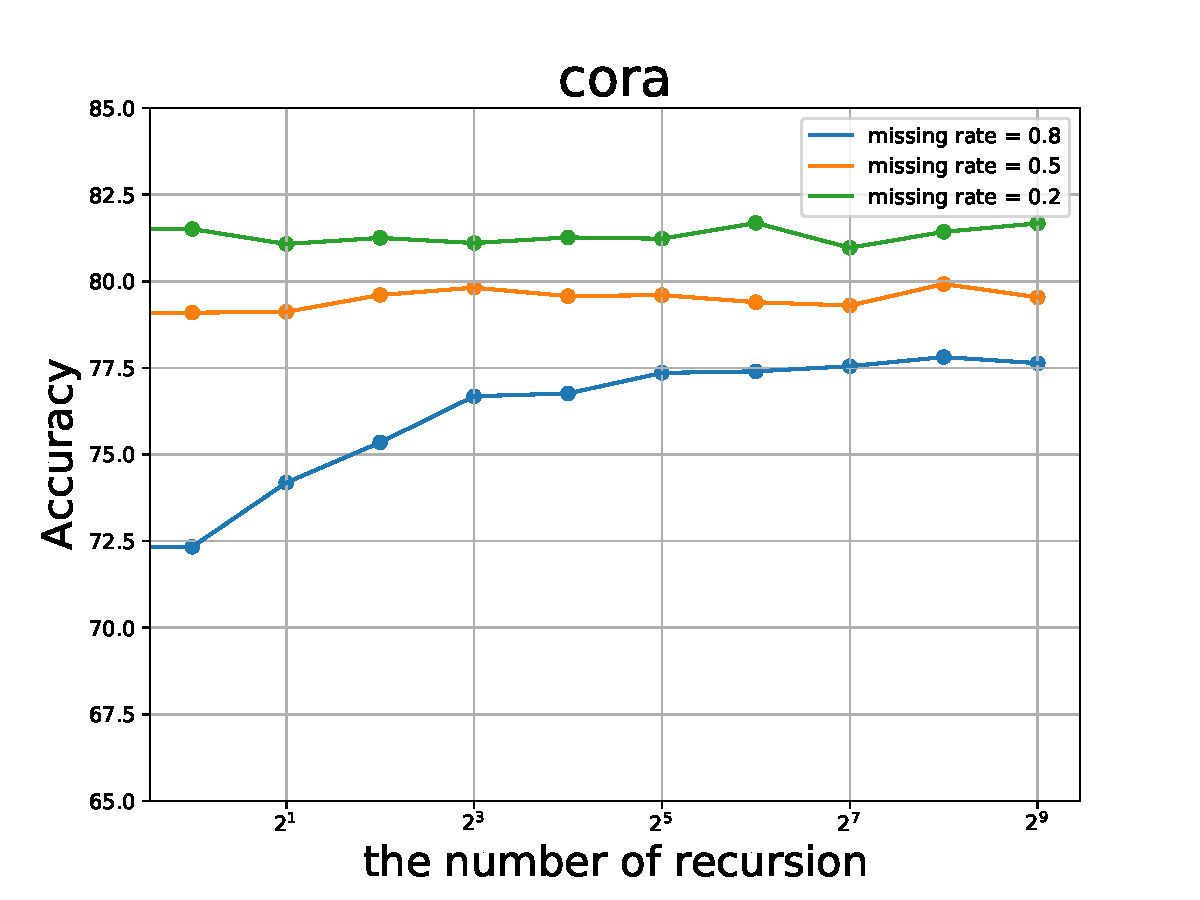
\includegraphics[clip, width=0.33\columnwidth]{figures/uniform_cora.pdf}}%
	\subfigure[Biased randomly missing]{%
		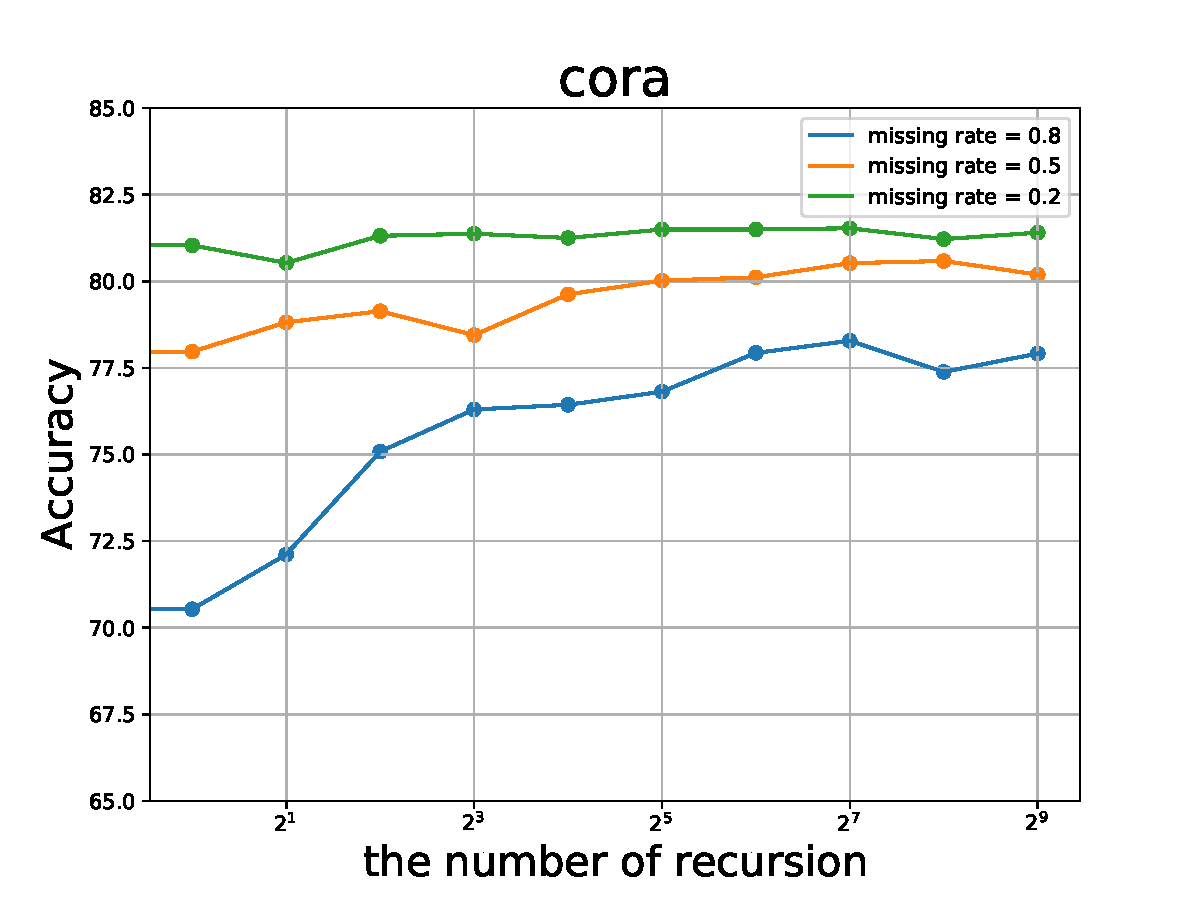
\includegraphics[clip, width=0.33\columnwidth]{figures/bias_cora.pdf}}%
    \subfigure[Structurally missing]{%
		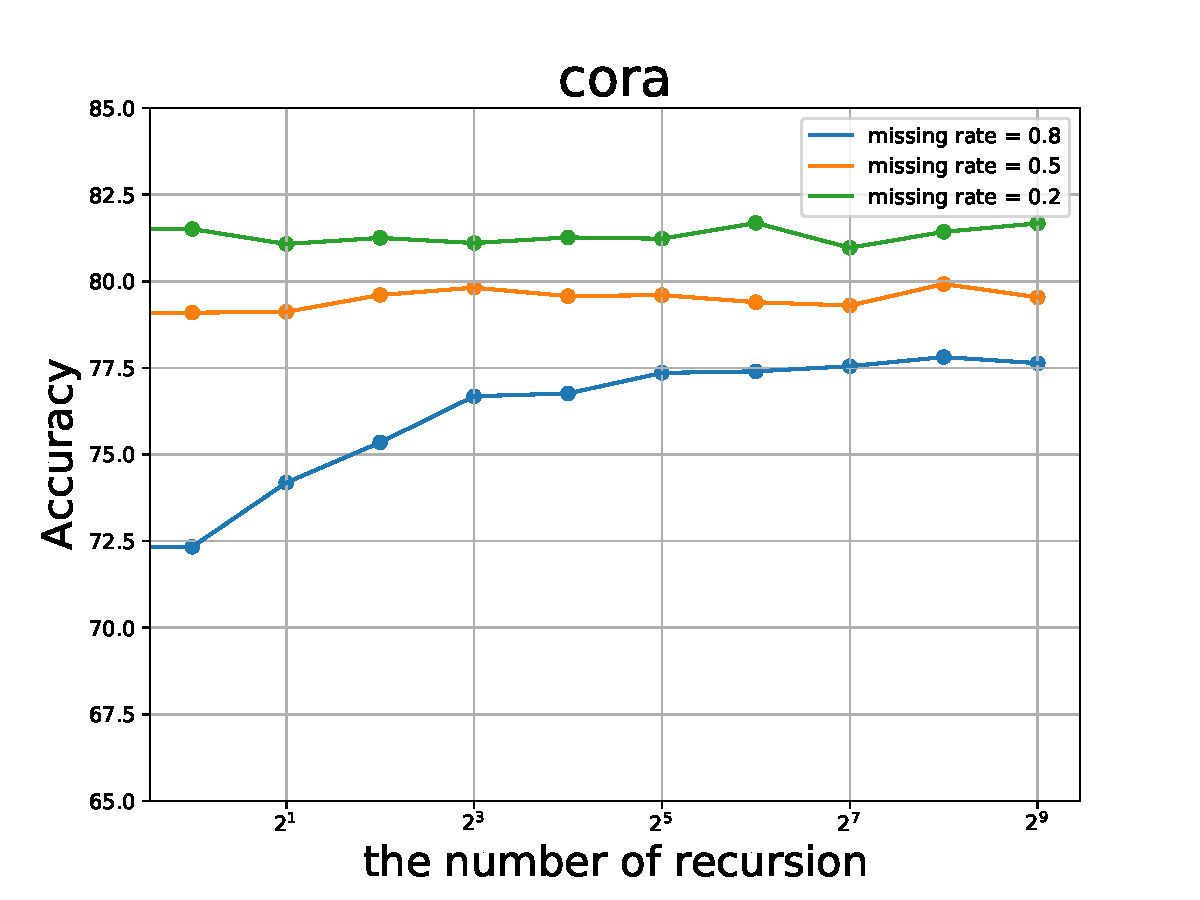
\includegraphics[clip, width=0.33\columnwidth]{figures/struct_cora.pdf}}%
	\caption{Coraでの分類精度}
	\label{fig:rec_cora}
\end{figure}

\begin{figure}
	\subfigure[Uniform randomly missing]{%
		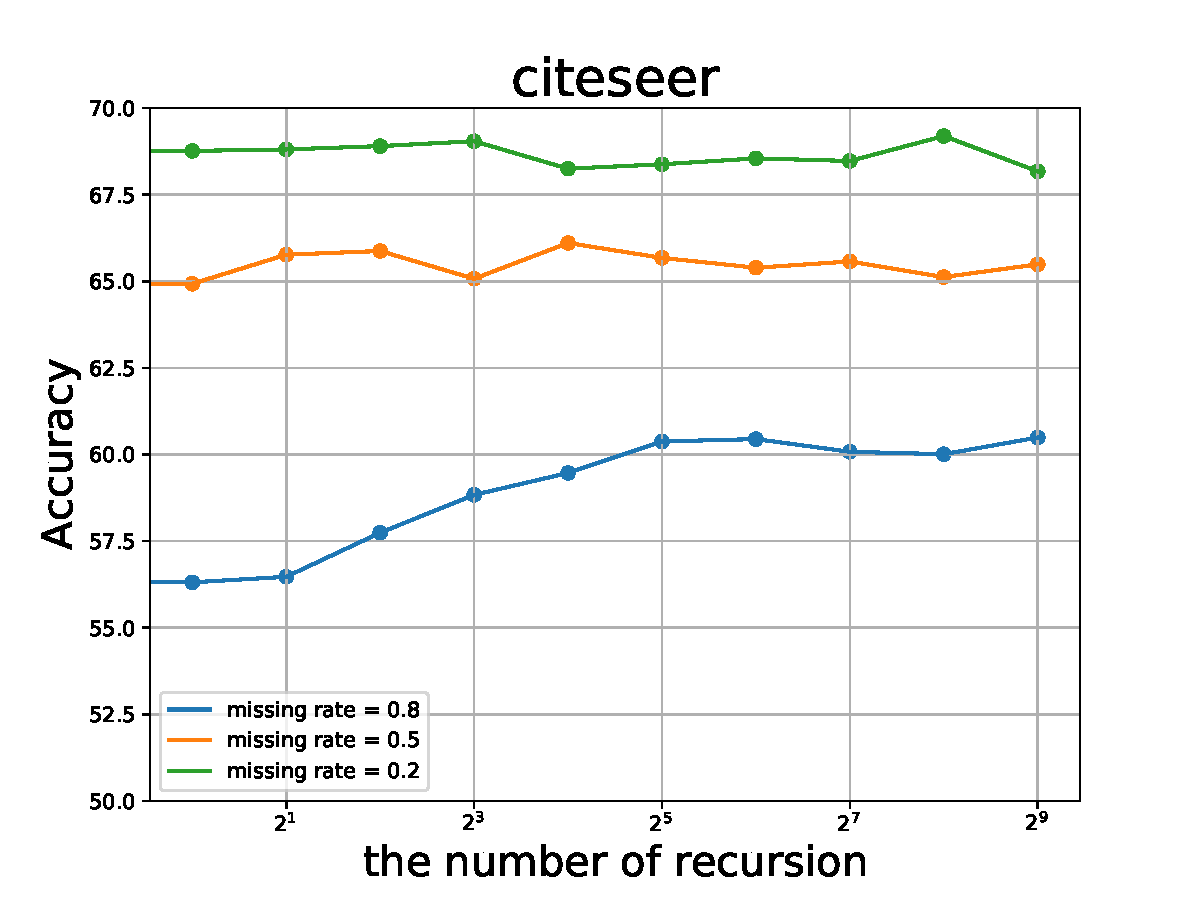
\includegraphics[clip, width=0.33\columnwidth]{figures/uniform_citeseer.pdf}}%
	\subfigure[Biased randomly missing]{%
		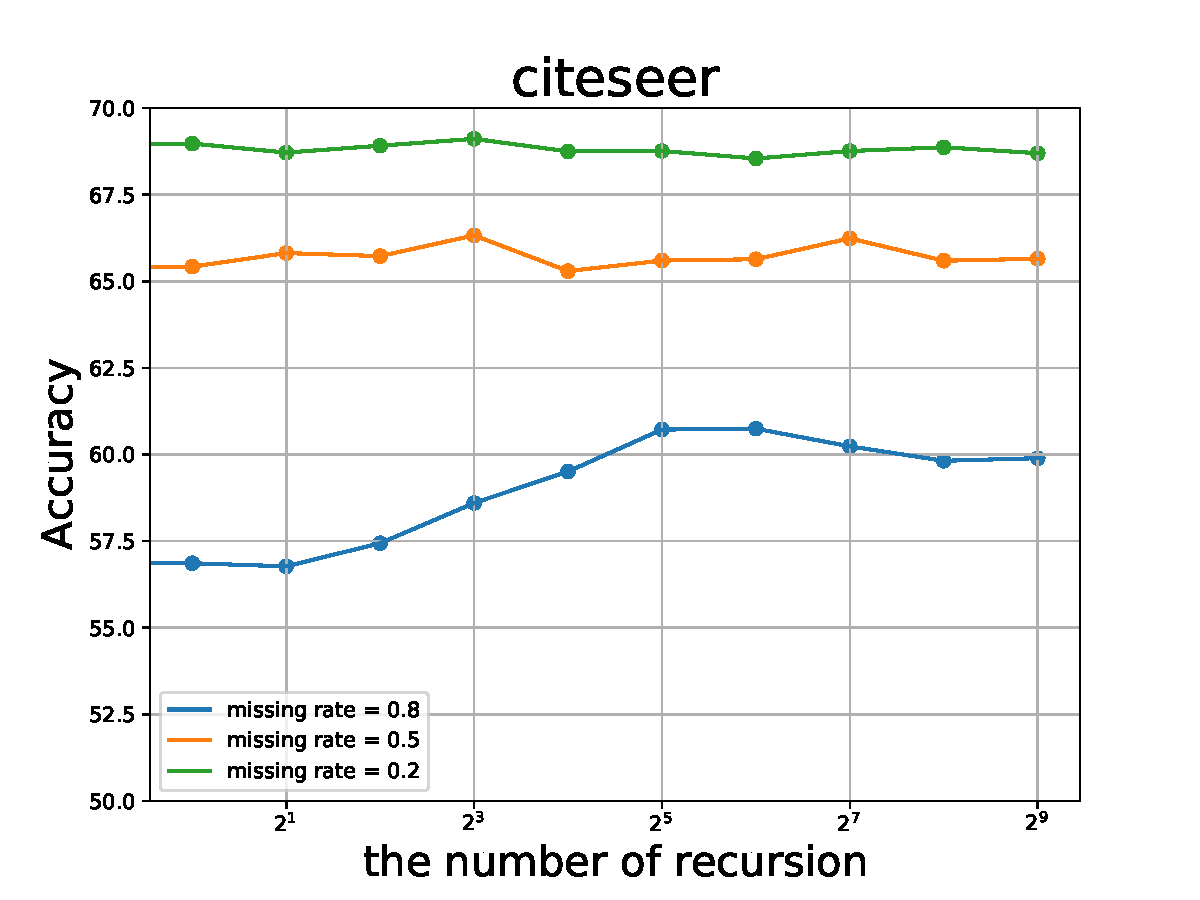
\includegraphics[clip, width=0.33\columnwidth]{figures/bias_citeseer.pdf}}%
    \subfigure[Structurally missing]{%
		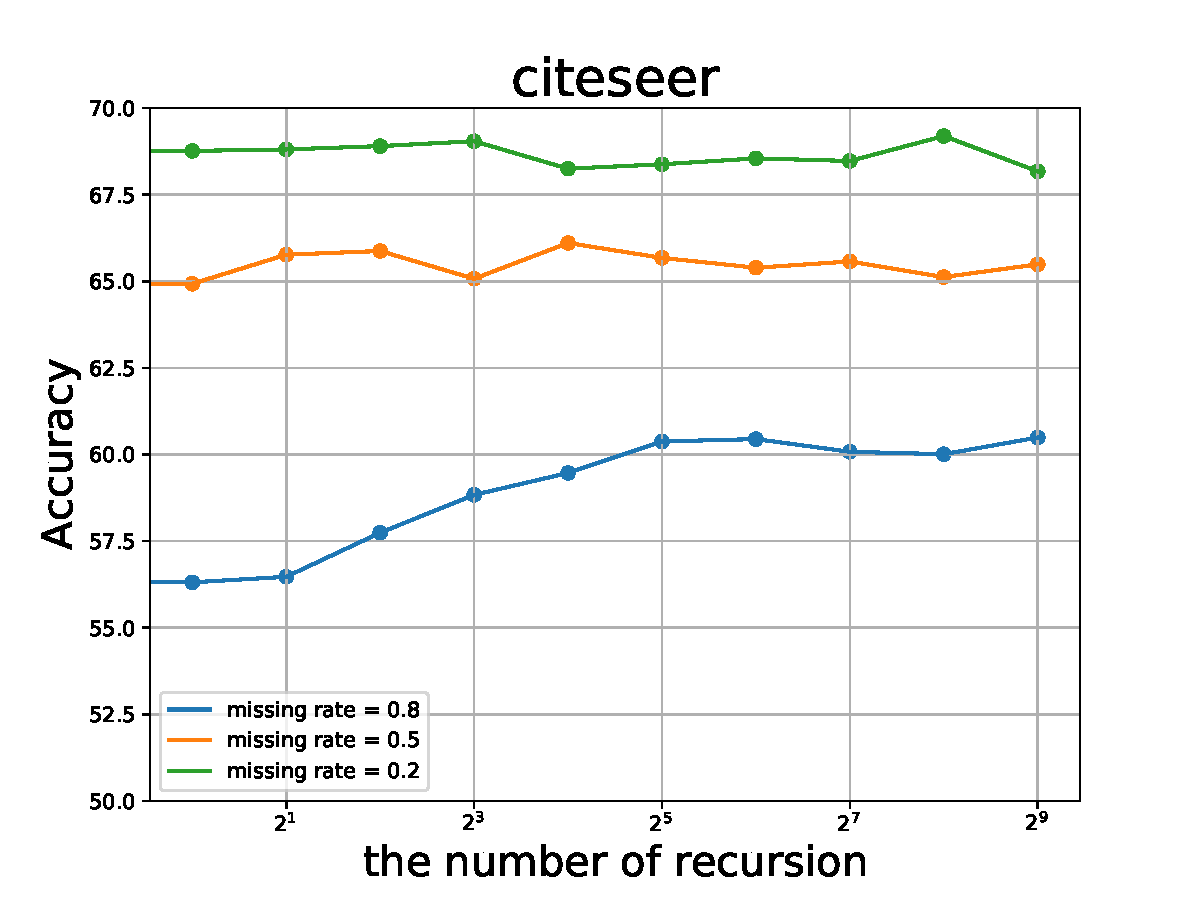
\includegraphics[clip, width=0.33\columnwidth]{figures/struct_citeseer.pdf}}%
	\caption{Citeseerでの分類精度}
	\label{fig:rec_citeseer}
\end{figure}

\begin{figure}
	\subfigure[Uniform randomly missing]{%
		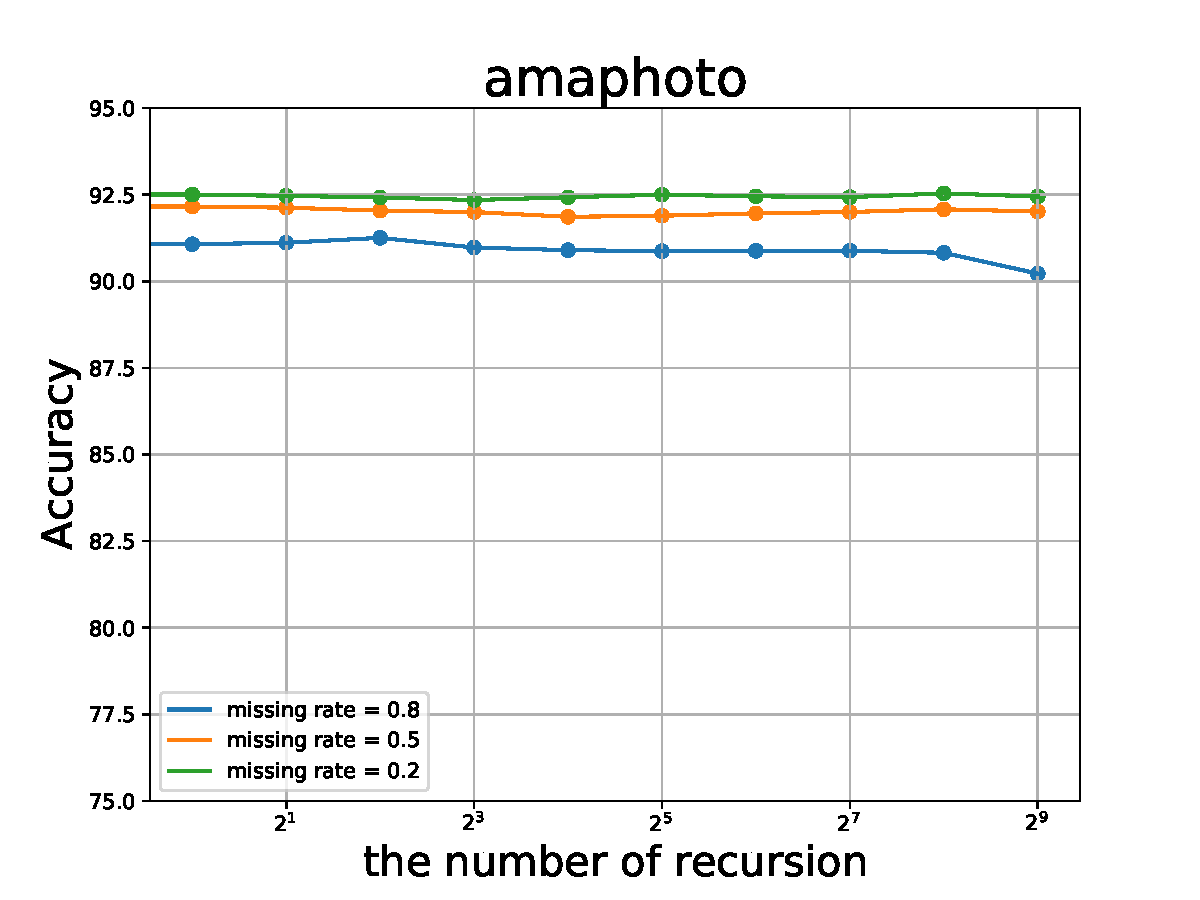
\includegraphics[clip, width=0.33\columnwidth]{figures/uniform_amaphoto.pdf}}%
	\subfigure[Biased randomly missing]{%
		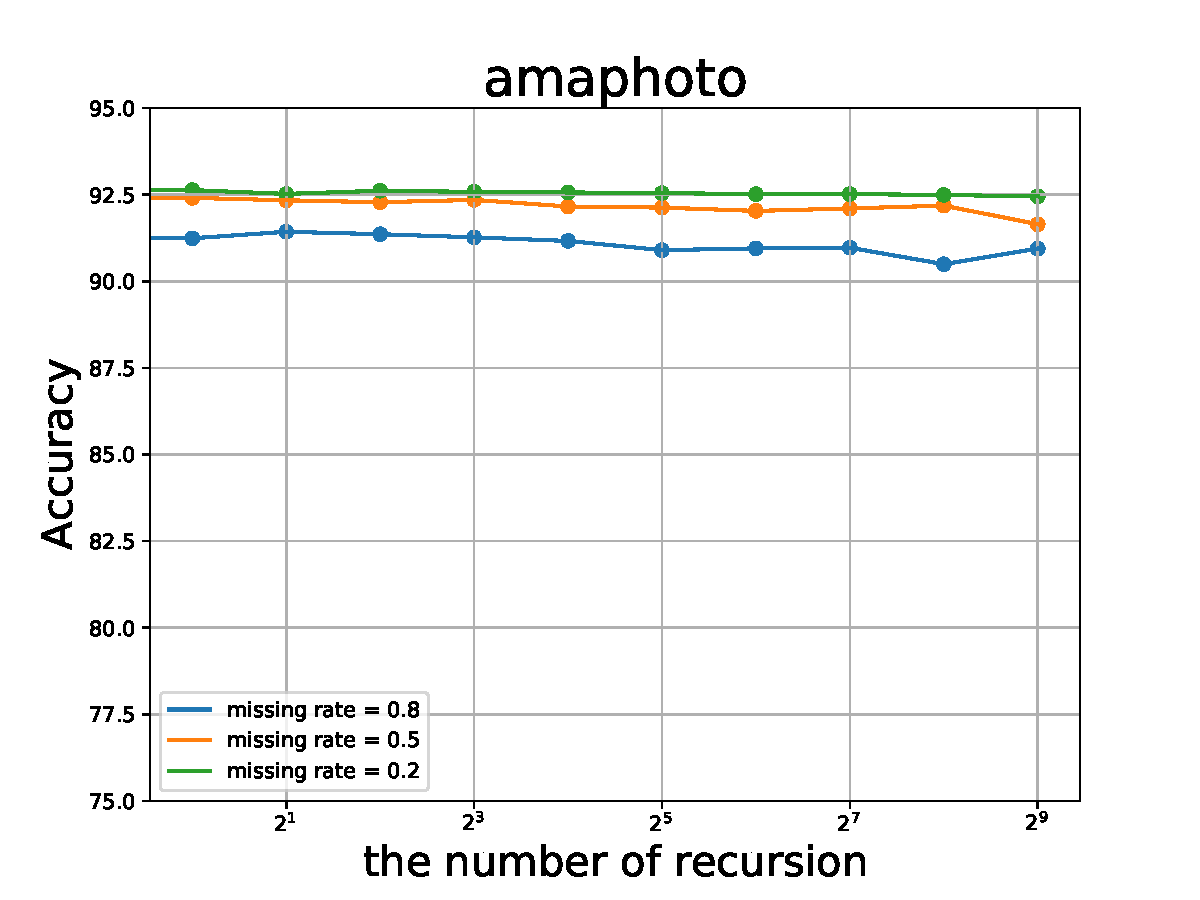
\includegraphics[clip, width=0.33\columnwidth]{figures/bias_amaphoto.pdf}}%
    \subfigure[Structurally missing]{%
		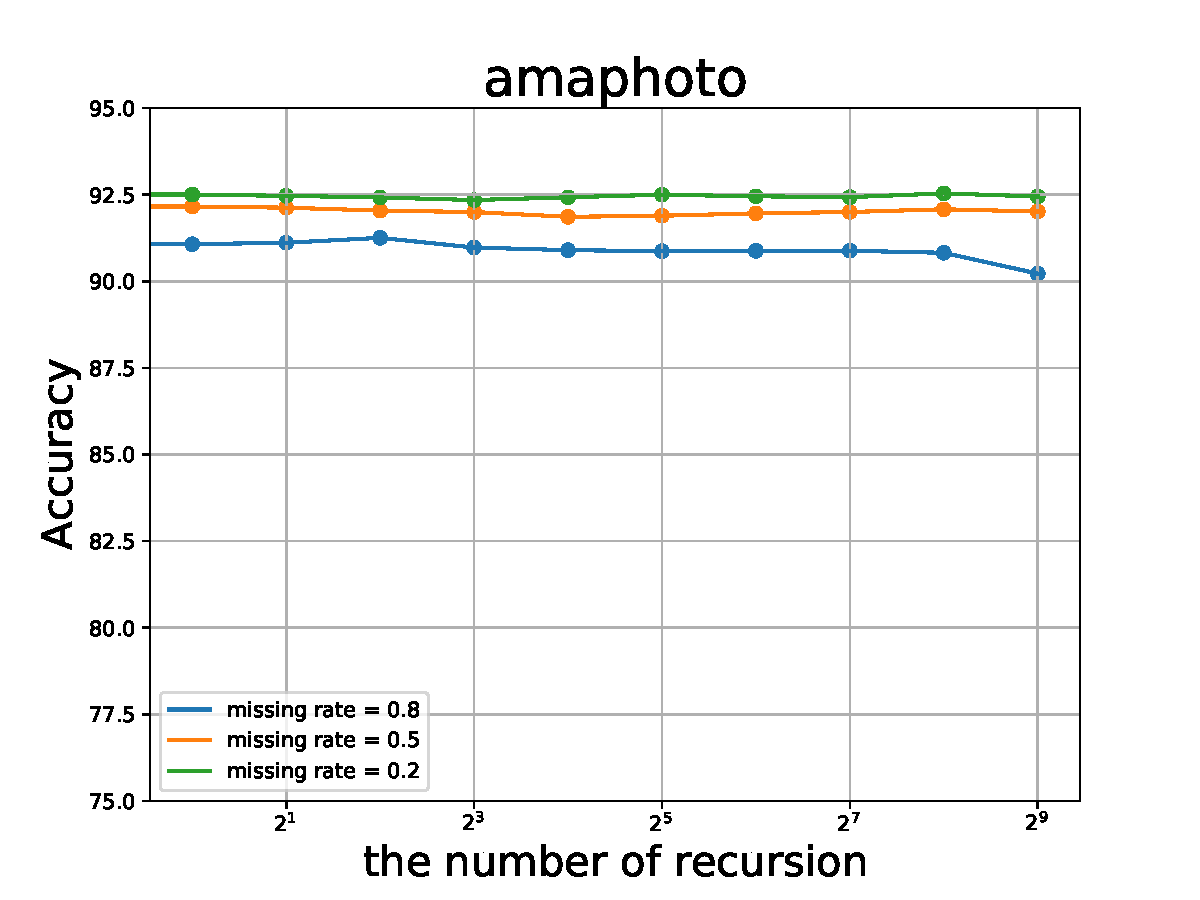
\includegraphics[clip, width=0.33\columnwidth]{figures/struct_amaphoto.pdf}}%
	\caption{Amaphotoでの分類精度}
	\label{fig:rec_amaphoto}
\end{figure}

\begin{figure}
	\subfigure[Uniform randomly missing]{%
		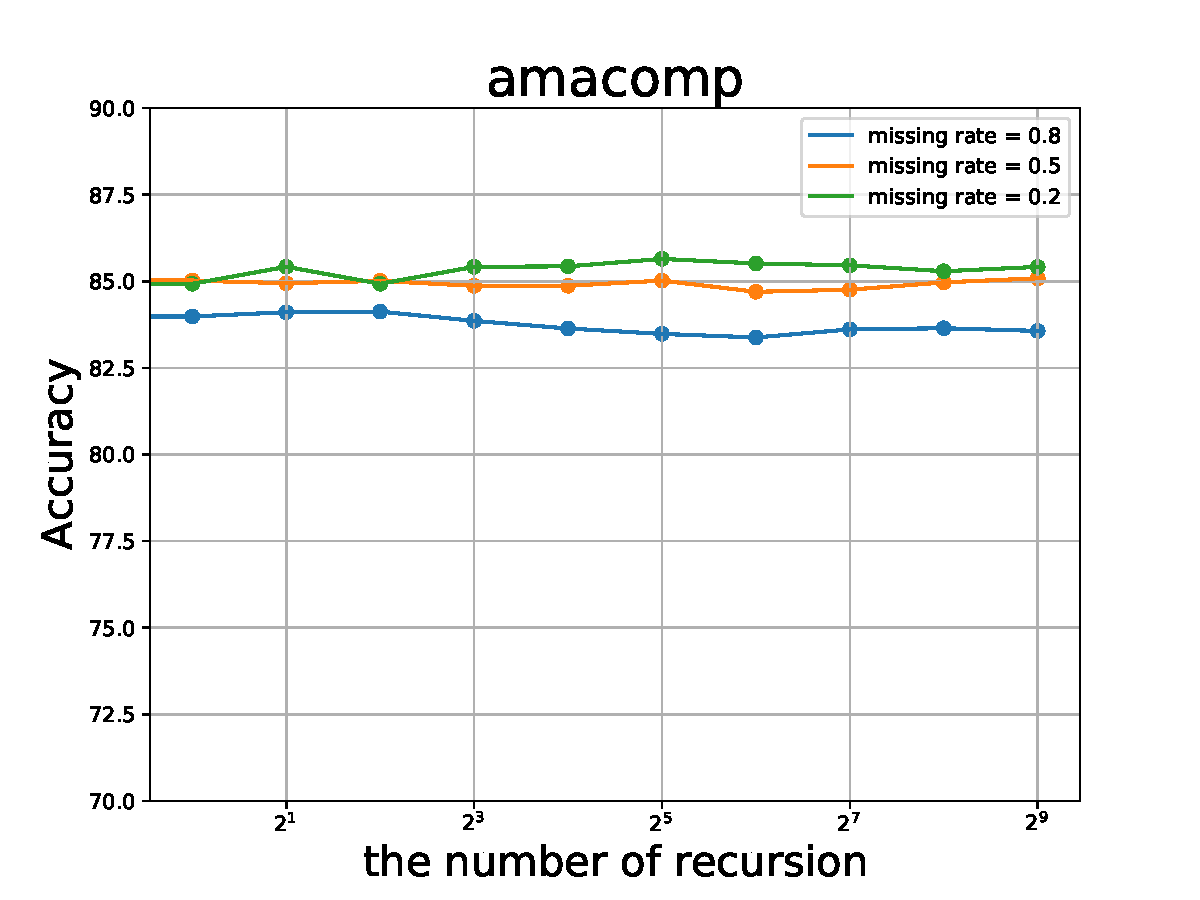
\includegraphics[clip, width=0.33\columnwidth]{figures/uniform_amacomp.pdf}}%
	\subfigure[Biased randomly missing]{%
		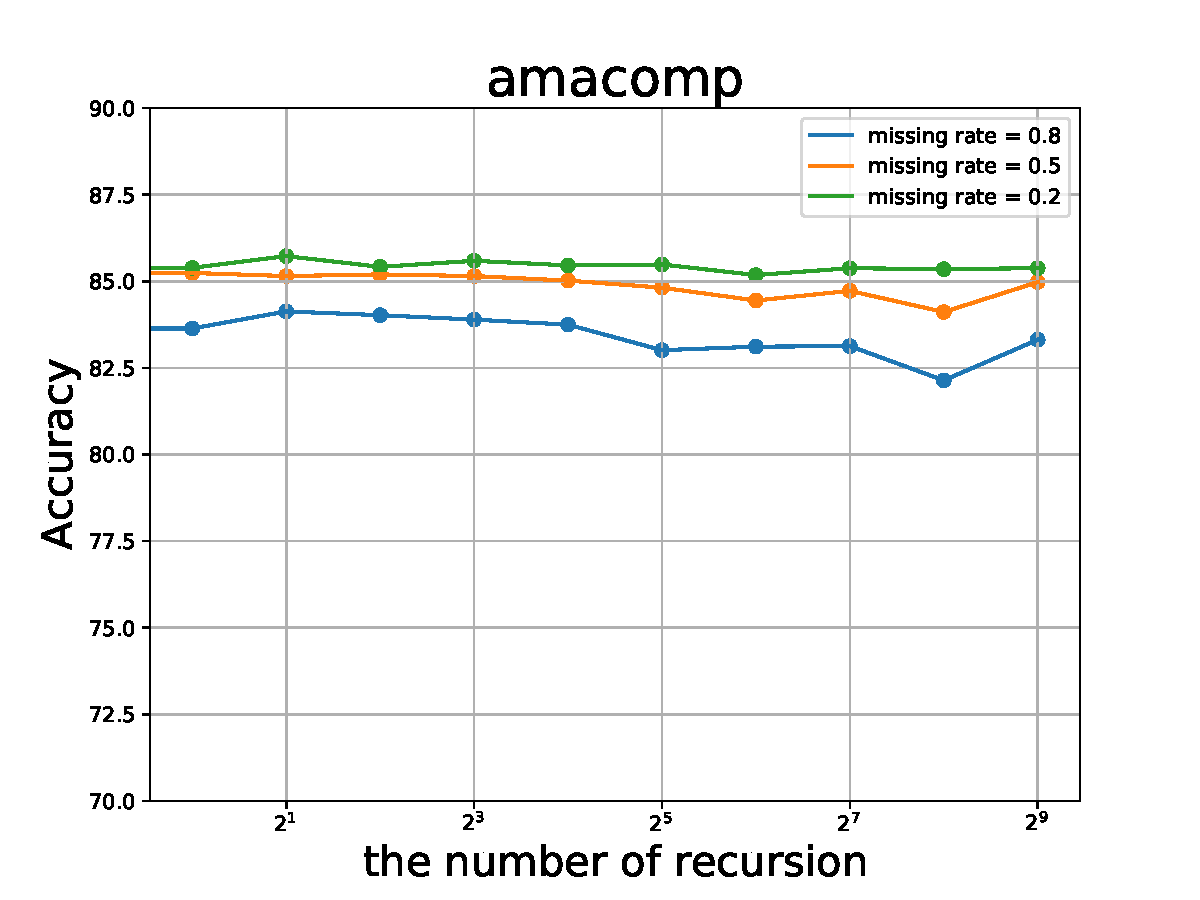
\includegraphics[clip, width=0.33\columnwidth]{figures/bias_amacomp.pdf}}%
    \subfigure[Structurally missing]{%
		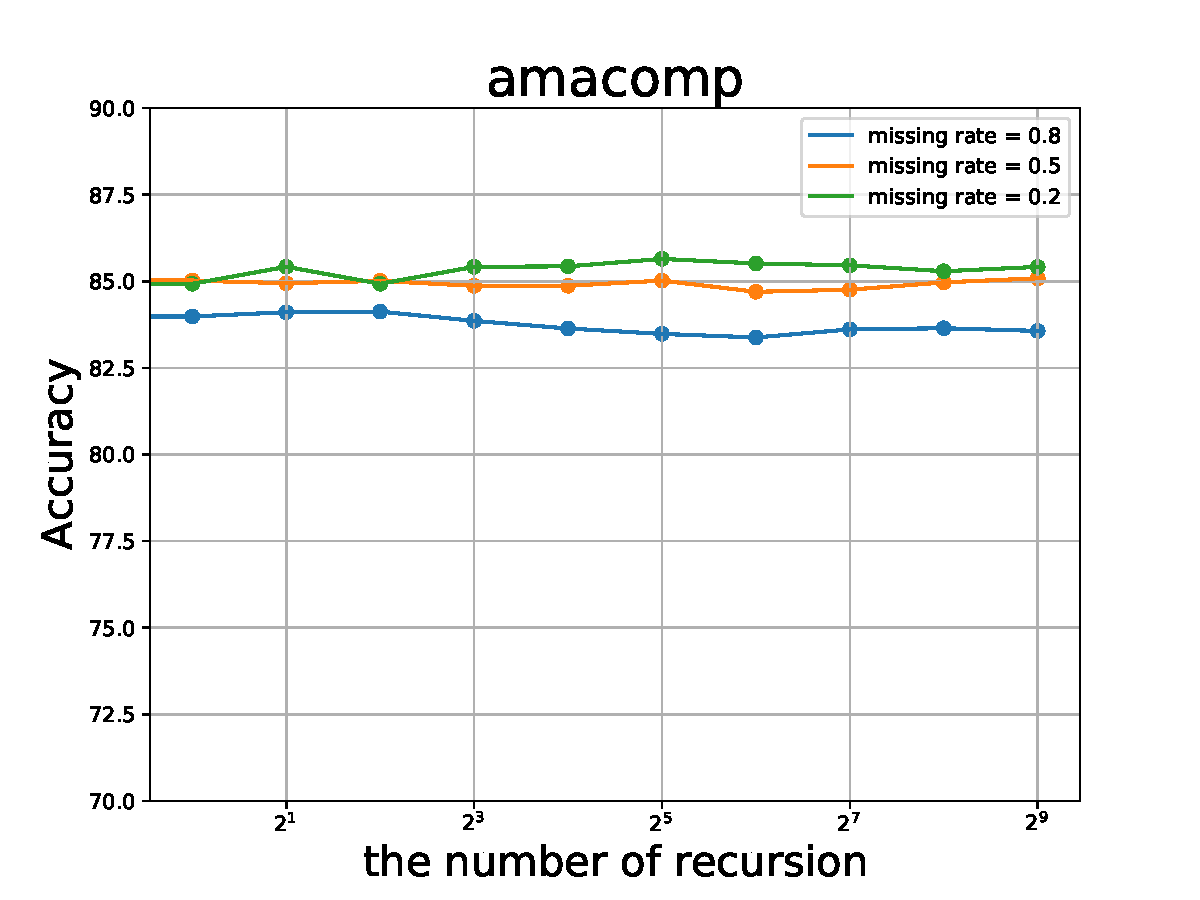
\includegraphics[clip, width=0.33\columnwidth]{figures/struct_amacomp.pdf}}%
	\caption{Amacompでの分類精度}
	\label{fig:rec_amacomp}
\end{figure}

\section{リンク予測}
提案手法の評価を行うためにリンク予測の精度を調べた。実験はノード分類と同様にUniform randomly missing, Biased randomly missing, Structurally missingの3種類の欠損パターンを用いた。また、欠損率は10\%から90\%までを10\%づつ変化させて9種類のパターンを用いた。また訓練/検証/テストエッジのデータセットの分割においては比較手法と同様に、全体のエッジから10\%を訓練エッジに、5\%を検証エッジに、残りの85\%をテストエッジにランダムに選択し決定した。また、訓練エッジとテストエッジにおいては正例のエッジと等しい数の負例のエッジをエッジが存在しないノードペア間からランダムに選択した。また実験は1つの欠損パターンで20回の実験を行い、それを5つの欠損パターンの平均で精度を調べた。つまり合計で100回の実験の平均をリンク予測の精度とした。

リンク予測の指標はエッジの正例と負例の判定をROC-AUCスコアとして求めた。この指標は0から100までの値をとり、値が大きいほど精度が良いことを示す。比較手法と同様の設定にするために、実験のエポック数を200、学習率を0.01とした。またGCNを用いる手法において隱れ層の次元数は32、潜在変数の次元を16に設定して実験を行った。また提案手法の1つであるGCN\_recursiveモデルの再帰回数は32回として実験を行った。

表\ref{table:linkcora}と表\ref{table:linkciteseer}ではデータセットCora,Citeseerにおけるリンク予測の精度を示している。各セルには手法、欠損パターン、欠損率ごとのROC-AUCスコアを示しており、太字の数字は、その欠損パターンと欠損率において最も精度が高いことを示している。提案手法は比較手法と比べると欠損率が低い場合はあまり精度が高くないといえる。しかし欠損率が高い場合は提案手法の1つであるGCN\_recursiveモデルは比較手法と比べて優れた精度を達成していることが確認できた。具体的にはデータセットCoraにおいては全ての欠損パターンにおいて欠損率90\%の場合に提案手法が比較手法よりも高い精度を達成しており、さらにデータセットCiteseerにおいてはStructurally missingの欠損パターンにおいて比較手法を上回っている。

半教師ありノード分類と異なり、提案手法が欠損率が低い場合に精度が低い理由は、提案手法がGCNに適した代入法を用いているために、リンク予測で扱うVGAEを用いたデコードに不向きな方法であるからであると考えられる。また提案手法GCN\_recursiveが欠損率が高い場合に精度が高い理由は、グラフ構造を用いて再帰的に特徴量を補完しているため、欠損率が高くても欠損率が低い場合と比べて欠損している特徴量を補完する精度があまり下がらず、その結果リンク予測精度を維持できているからであると考えられる。

\label{sec:linkpred}

\begin{table}[!p]
    \centering
    \caption{Coraデータセットにおけるリンク予測のROC-AUCスコア}
    \label{table:linkcora}
    \scalebox{.84}{
    \begin{tabular}{c|c|ccccccccc} \toprule
欠損パターン &  欠損率 & 10\% & 20\% & 30\% & 40\% & 50\% & 60\% & 70\% & 80\% & 90\%\\ \midrule
\multirow{13}{*}{\shortstack{Uniform\\Randomly\\Missing}} & \textsc{Mean} & 90.72 & 90.41 & 90.10 & 89.79 & 89.11 & 88.40 & 87.13 & 84.47 & 74.97\\
& \textsc{K-NN} & 92.20 & 91.86 & 91.34 & 90.93 & 90.19 & 89.03 & 87.62 & 85.69 & 81.55\\
& \textsc{MFT} & 92.16 & 91.86 & 91.37 & 90.91 & 90.14 & 88.37 & 86.11 & 84.10 & 79.94\\
& \textsc{SoftImp} & 90.88 & 90.79 & 90.64 & 90.40 & 89.98 & 89.22 & 88.37 & 86.75 & {84.13}\\
& \textsc{MICE} & -- & -- & -- & -- & -- & -- & -- & -- & --\\
& \textsc{MissForest} & {92.32} & \underline{92.04} & 91.61 & 90.95 & 90.33 & 89.34 & 88.33 & 86.41 & 82.78\\
& \textsc{VAE} & 92.23 & 91.91 & 91.33 & 90.54 & 89.28 & 86.98 & 82.52 & 77.74 & 77.27\\
& \textsc{GAIN} & 92.17 & 91.87 & 91.46 & {91.00} & {90.57} & {89.78} & {89.17} & {88.13} & 86.01\\
& \textsc{GINN} & 92.15 & 91.96 & {91.62} & {91.00} & 90.28 & 88.94 & 87.66 & 84.73 & 74.90\\
& \textsc{GCNmf} & \textbf{94.09} & \textbf{93.50} & \textbf{93.05} & \textbf{92.40} & \textbf{92.29} & \textbf{91.79} & \textbf{90.77} & \textbf{88.32} & 81.46\\ 
& \textsc{GCN\_neighbor} & 90.84 & 90.06 & 89.69 & 89.16 & 88.47 & 88.44 & 87.77 & 86.54 & 86.05 \\
& \textsc{GCN\_recursive} & 90.41 & 90.53 & 90.06 & 89.45 & 89.68 & 88.07 & 88.65 & 87.38 & \textbf{87.14} \\
\midrule
\multirow{13}{*}{\shortstack{Biased\\Randomly\\Missing}} & \textsc{Mean} & 92.18 & 92.08 & 92.14 & 91.89 & 91.43 & 91.01 & 89.55 & 87.19 & 76.96\\
& \textsc{K-NN} & 92.17 & 92.06 & 92.02 & 91.83 & 91.47 & 90.92 & 89.84 & 87.85 & 81.65\\
& \textsc{MFT} & 92.17 & 91.44 & 90.65 & 90.00 & 89.50 & 88.91 & 87.48 & 85.36 & 80.20\\
& \textsc{SoftImp} & {92.35} & {92.34} & {92.35} & {92.08} & {91.74} & {91.36} & \textbf{90.03} & {88.44} & {86.17}\\
& \textsc{MICE} & -- & -- & -- & -- & -- & -- & -- & -- & --\\
& \textsc{MissForest} & 92.27 & 92.22 & 92.22 & 91.80 & 91.22 & 90.34 & 88.90 & 86.86 & 83.58\\
& \textsc{VAE} & 92.19 & 92.05 & 91.83 & 91.37 & 90.75 & 89.71 & 87.37 & 84.95 & 76.71\\
& \textsc{GAIN} & 92.18 & 92.01 & 91.88 & 91.70 & 91.28 & 90.75 & {89.87} & \textbf{88.75} & 86.69\\
& \textsc{GINN} & 92.15 & 92.11 & 92.04 & 91.88 & 91.52 & 90.89 & 89.45 & 87.36 & 75.38\\
& \textsc{GCNmf} & \textbf{94.35} & \textbf{94.20} & \textbf{93.90} & \textbf{93.15} & \textbf{92.43} & \textbf{91.46} & \textbf{90.03} & 86.10 & 81.72\\ 
& \textsc{GCN\_neighbor}  & 90.26 & 89.73 & 90.35 & 89.68 & 89.66 & 89.07 & 87.69 & 85.93 & 86.36 \\
& \textsc{GCN\_recursive} & 90.00 & 89.53 & 88.85 & 89.18 & 88.79 & 87.58 & 87.13 & 87.29 & \textbf{86.94} \\
\midrule
\multirow{13}{*}{\shortstack{Structurally\\Missing}} & \textsc{Mean} & 90.34 & 89.79 & 89.12 & 88.26 & 87.12 & 85.33 & 83.23 & 79.61 & 71.79\\
& \textsc{K-NN} & {91.60} & 91.08 & {90.38} & {89.36} & {88.34} & 87.16 & 85.40 & 82.09 & 76.12\\
& \textsc{MFT} & 91.51 & 91.00 & 89.95 & 89.11 & 87.36 & 85.81 & 82.90 & 77.73 & 73.72\\
& \textsc{SoftImp} & 90.29 & 89.67 & 88.86 & 87.86 & 86.77 & 85.36 & 83.07 & {81.53} & 77.38\\
& \textsc{MICE} & 91.58 & {91.11} & 90.30 & 89.34 & 88.18 & {86.70} & {84.24} & 80.31 & 72.63\\
& \textsc{MissForest} & 91.57 & 91.05 & 90.23 & {89.36} & {88.34} & 87.16 & 85.40 & 82.09 & {76.22}\\
& \textsc{VAE} & 91.49 & 90.76 & 89.49 & 87.27 & 83.81 & 80.07 & 73.46 & 67.55 & 65.80\\
& \textsc{GAIN} & {91.60} & 91.08 & {90.38} & {89.36} & {88.34} & 87.16 & 85.40 & 82.09 & 76.12\\
& \textsc{GINN} & 91.51 & 90.85 & 89.68 & 87.34 & 83.23 & 76.22 & 66.55 & 63.88 & 64.91\\
& \textsc{GCNmf} & \textbf{93.55} & \textbf{92.65} & \textbf{91.68} & \textbf{90.55} & \textbf{88.54} & 86.19 & 81.96 & 76.35 & 67.86\\ 
& \textsc{GCN\_neighbor} & 91.03 & 89.74 & 89.55 & 88.73 & 87.90 & 86.71 & 85.47 & 84.12 & 79.78 \\
& \textsc{GCN\_recursive} & 89.52 & 89.40 & 89.01 & 88.44 & 88.47 & \textbf{87.26} & \textbf{87.30} & \textbf{86.66} & \textbf{85.20} \\
\midrule
\multicolumn{2}{c|}{GCN}& \multicolumn{9}{c}{92.42}\\
\multicolumn{2}{c|}{GCN $(\mathbf{X} = \mathbf{I}_N)$}& \multicolumn{9}{c}{85.90}\\ 
\bottomrule
    \end{tabular}
    }
\end{table}

\begin{table}[!p]
    \centering
    \caption{Citeseerデータセットにおけるリンク予測のROC-AUCスコア}
    \label{table:linkciteseer}
    \scalebox{.84}{
    \begin{tabular}{c|c|ccccccccc} \toprule
欠損パターン &  欠損率 & 10\% & 20\% & 30\% & 40\% & 50\% & 60\% & 70\% & 80\% & 90\%\\ \midrule
\multirow{13}{*}{\shortstack{Uniform\\Randomly\\Missing}} & \textsc{Mean} & 89.01 & 88.56 & 88.01 & 87.33 & 86.42 & 85.30 & 83.77 & 81.43 & 75.47\\
& \textsc{K-NN} & 90.00 & 89.60 & 89.10 & 88.34 & 87.32 & 85.68 & 83.39 & 81.16 & 78.60\\
& \textsc{MFT} & 89.86 & 89.43 & 88.81 & 87.72 & 85.76 & 83.24 & 81.20 & 79.97 & 77.94\\
& \textsc{SoftImp} & {90.19} & {90.15} & {89.81} & {89.55} & {88.97} & {88.17} & {86.80} & {84.99} & 81.66\\
& \textsc{MICE} & -- & -- & -- & -- & -- & -- & -- & -- & --\\
& \textsc{MissForest} & -- & -- & -- & -- & -- & -- & -- & -- & --\\
& \textsc{VAE} & 89.85 & 89.09 & 88.13 & 87.22 & 85.36 & 83.55 & 80.64 & 74.89 & 64.69\\
& \textsc{GAIN} & 89.96 & 89.53 & 89.07 & 88.36 & 87.51 & 86.52 & 85.35 & 83.93 & {81.70}\\
& \textsc{GINN} & 90.02 & 89.64 & 89.04 & 87.91 & 86.56 & 84.64 & 83.32 & 81.82 & 77.19\\
& \textsc{GCNmf} & \textbf{93.20} & \textbf{92.96} & \textbf{92.30} & \textbf{92.19} & \textbf{90.45} & \textbf{90.08} & \textbf{88.91} & \textbf{87.28} & \textbf{83.68}\\ 
& \textsc{GCN\_neighbor} & 89.00 & 87.14 & 86.02 & 85.20 & 84.32 & 83.48 & 82.92 & 81.51 & 81.36 \\
& \textsc{GCN\_recursive} & 88.23 & 87.47 & 87.17 & 86.20 & 86.65 & 85.12 & 83.54 & 83.26 & 81.70\\
\midrule
\multirow{13}{*}{\shortstack{Biased\\Randomly\\Missing}} & \textsc{Mean} & 89.94 & 89.88 & 89.63 & 89.33 & 89.25 & 88.55 & {87.57} & 85.28 & 78.23\\
& \textsc{K-NN} & 90.00 & 89.98 & 89.81 & 89.54 & 89.31 & 88.52 & 87.47 & 84.97 & 78.85\\
& \textsc{MFT} & 89.98 & 87.50 & 85.88 & 85.07 & 84.32 & 83.76 & 82.85 & 81.54 & 78.23\\
& \textsc{SoftImp} & {90.31} & {90.25} & {90.23} & {89.99} & {89.90} & {89.03} & 87.12 & {85.96} & 80.63\\
& \textsc{MICE} & -- & -- & -- & -- & -- & -- & -- & -- & --\\
& \textsc{MissForest} & -- & -- & -- & -- & -- & -- & -- & -- & --\\
& \textsc{VAE} & 89.90 & 89.25 & 88.33 & 87.32 & 86.26 & 83.78 & 83.05 & 80.71 & 62.51\\
& \textsc{GAIN} & 89.97 & 89.87 & 89.60 & 89.32 & 88.89 & 87.85 & 87.00 & 85.05 & \textbf{81.95}\\
& \textsc{GINN} & 90.27 & 89.99 & 89.85 & 89.47 & 89.10 & 88.15 & 87.21 & 84.47 & 76.83\\
& \textsc{GCNmf} & \textbf{93.53} & \textbf{93.38} & \textbf{92.81} & \textbf{92.48} & \textbf{91.68} & \textbf{91.25} & \textbf{89.54} & \textbf{86.73} & {81.43}\\ 
& \textsc{GCN\_neighbor} & 88.36 & 87.67 & 86.81 & 85.71 & 85.39 & 83.40 & 83.17 & 81.71 & 80.20 \\
& \textsc{GCN\_recursive} & 89.53 & 88.31 & 87.47 & 87.16 & 85.60 & 84.27 & 84.58 & 82.21 & 80.89 \\
\midrule
\multirow{13}{*}{\shortstack{Structurally\\Missing}} & \textsc{Mean} & 88.16 & 86.95 & 85.76 & 84.20 & 82.43 & 80.83 & 78.92 & 75.79 & 69.76\\
& \textsc{K-NN} & {89.50} & {88.36} & {87.01} & {85.52} & {83.85} & {82.11} & {79.81} & {76.49} & 70.86\\
& \textsc{MFT} & 89.24 & 87.96 & 86.53 & 84.76 & 83.19 & 80.67 & 78.35 & 75.97 & {72.64}\\
& \textsc{SoftImp} & {89.50} & {88.36} & {87.01} & {85.52} & {83.85} & {82.11} & {79.81} & {76.49} & 70.86\\
& \textsc{MICE} & -- & -- & -- & -- & -- & -- & -- & -- & --\\
& \textsc{MissForest} & -- & -- & -- & -- & -- & -- & -- & -- & --\\
& \textsc{VAE} & 88.57 & 86.83 & 84.32 & 80.96 & 77.49 & 74.01 & 67.84 & 63.06 & 60.39\\
& \textsc{GAIN} & {89.50} & {88.36} & {87.01} & {85.52} & {83.85} & {82.11} & {79.81} & {76.49} & 70.86\\
& \textsc{GINN} & 87.48 & 83.35 & 77.50 & 70.06 & 64.31 & 59.45 & 57.95 & 54.88 & 50.81\\
& \textsc{GCNmf} & \textbf{92.23} & \textbf{90.54} & \textbf{88.77} & \textbf{85.74} & \textbf{84.78} & \textbf{84.59} & \textbf{82.00} & 77.21 & 73.31\\ 
& \textsc{GCN\_neighbor} & 88.27 & 87.06 & 86.18 & 84.89 & 82.93 & 80.78 & 79.93 & 79.03 & 74.37 \\
& \textsc{GCN\_recursive} & 88.45 & 87.38 & 86.60 & 84.61 & 82.94 & 81.97 & 81.03 & \textbf{79.04} & \textbf{79.40}\\
\midrule
\multicolumn{2}{c|}{GCN}& \multicolumn{9}{c}{90.25}\\
\multicolumn{2}{c|}{GCN $(\mathbf{X} = \mathbf{I}_N)$}& \multicolumn{9}{c}{79.94}\\ 
\bottomrule
    \end{tabular}
    }
\end{table}

